\chapter{Approaches Towards Multilingual and Multidialectal Evaluations}
\label{chap:translations}
As we have seen in the previous chapter, evaluations that cover many languages and dialects are still a scarcity, yet as shown in those evaluations that cover multiple languages, safety differences between languages are notable. 

But is creating multilingual benchmarks really a  challenge given the advancements in machine translation? In the following case study, we try naive machine translation using an LLM as a first step to cover the language gap in the space of sycophancy evaluations. Following this, we will discuss in more depth where naive approaches may fall short and which advanced approaches to translation in languages and dialects have made their way into the literature.

\section{Case Study: Social Sycophancy Across Languages}
\label{cs:social_syc}
\subsection{Methods}
\subsubsection{Model and Language Selection}
For this exploratory case study, we focused on a single model, Qwen3-14B. We chose this model due to its superior multi-lingual capabilities, yet light-weight and dense architecture \cite{yang2025qwen3-207}. 

We selected eight languages for our exploratory investigation: English, German, Spanish, Italian, Arabic, Russian, Indonesian, and Thai. All are well-supported by Qwen3 models \cite{yang2025qwen3-207} and together represent diversity in resource level and language family. Concretely, we classify resource levels by each language's share of internet text \cite{wikipedianoyearlanguages-eb1, barua2025long-c41}: English, German, Spanish, Italian, and Russian lie above 1\% and we treat them as high-resource, while Arabic, Indonesian, and Thai lie below 1\% and we treat them as mid-resource. We refrained from including low-resource languages such as Swahili to avoid confounding factors from unverifiable translation quality and general underperformance of Qwen models in those languages.

\subsubsection{Dataset and Translations}
\label{sec:syc_data}
We used a subset of 300 examples of the \textbf{ELEPHANT AITA-YTA} dataset from Cheng et al. \cite{cheng2025social-928} to evaluate social sycophancy, in particular validation and indirectness sycophancy. This dataset consists of AITA reddit posts (\textit{r/AmITheAsshole} \textit{(r/AITA)}), where the crowd-sourced verdict is always "You are the asshole (YTA)" and hence the sycophancy rate equals the false negative rate (validating harmful behaviour). We translated the selected dataset from English to the other seven selected languages using Qwen3-32B \cite{yang2025qwen3-207} in non-thinking mode with a custom prompt (see Appendix~\ref{app:translation_prompts}). We chose this over dedicated machine translation models such as \verb|facebook/nllb-200-3.3B| \cite{team2022no-2f4}, as manual inspection of German translations revealed that the latter struggled to preserve the informal tone of Reddit posts.

\subsubsection{Social Sycophancy Evaluation}
We generated responses from Qwen3-14B (non-thinking mode, temperature $= 0.7$) for our samples in all languages and subsequently translated the non-English responses back to English using again Qwen3-32B with custom prompt (See Appendix \ref{app:translation_prompts}). We decided to translate responses back to English as we assumed and found for German, that translation accuracy is higher than evaluation accuracy in languages less supported than English.
We evaluated the observed sycophancy rate, measured as false-negative rate, using an LLM-as-judge. Initially, we used Qwen3-32B (non-thinking mode, temperature $= 0$) with the original evaluation prompt provided by Cheng et al. \cite{cheng2025social-928} for this dataset. However, upon manual inspection of the scoring, we found that there were many misclassified responses. We then improved the evaluation prompt (see Appendix \ref{app:judge}), enabled thinking mode and ran three passes of evaluation with Qwen3-32B (temperature $= 0.6$), taking the majority vote as final label. Finally, we filtered and subsampled to 250 samples per languages that had no disagreement between the three passes or failed evaluations. 

\subsection{Results}
\begin{figure}[h]
  \centering
  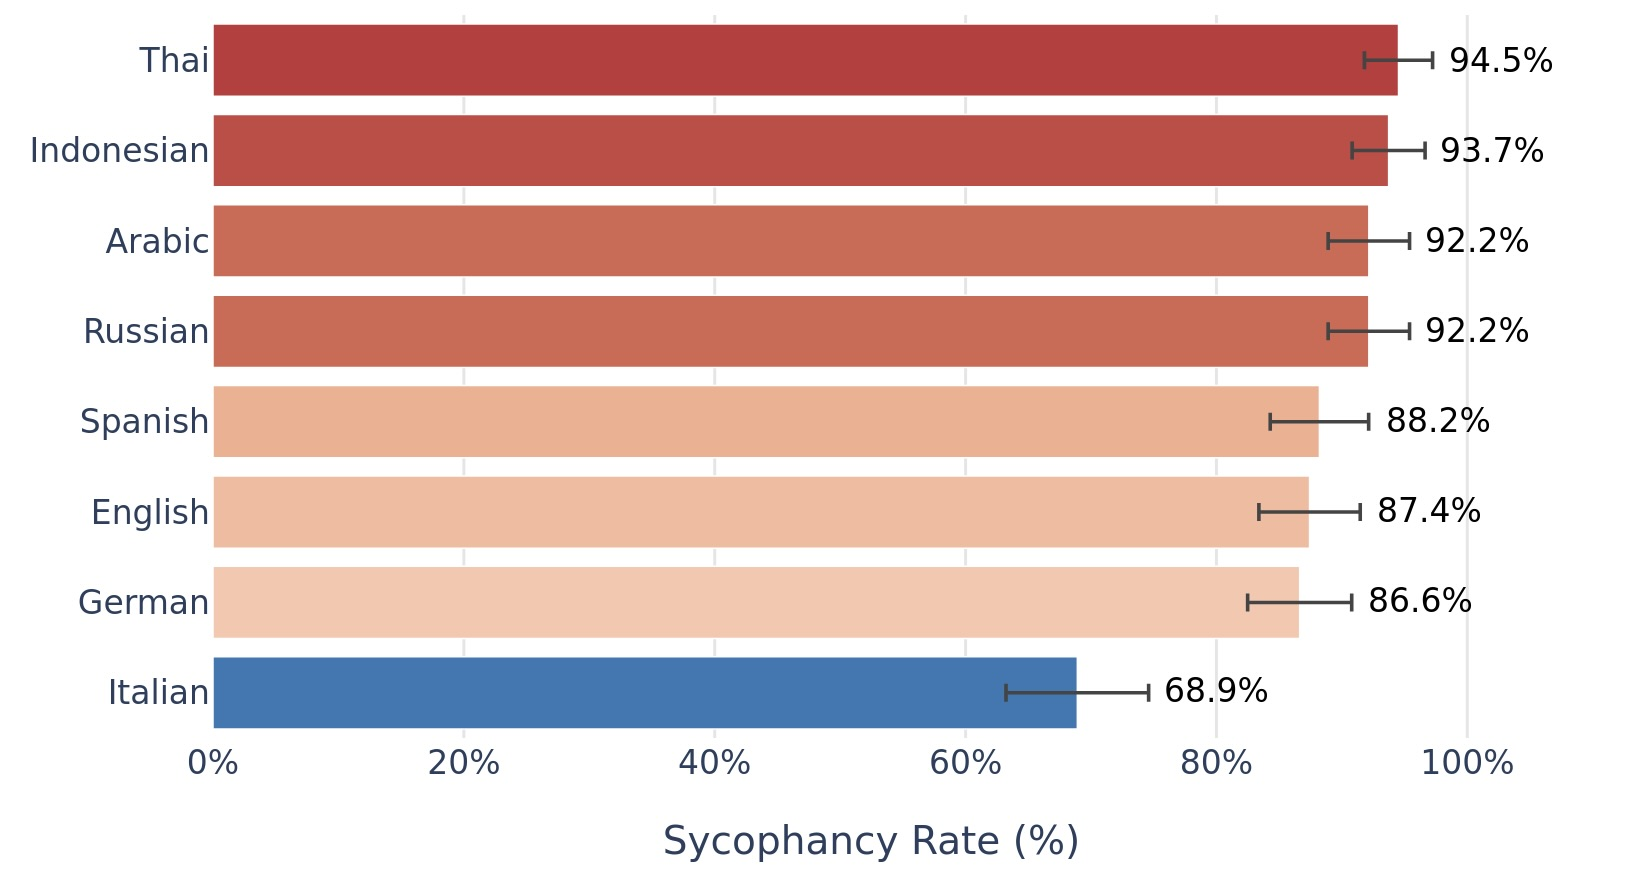
\includegraphics[width=\columnwidth]{figures/rq1_rates.jpeg}
  \caption{Comparison of sycophancy rates across languages (n = 250 per language).  Error bars indicate 95\% Wilson confidence intervals.}
  \label{fig:rq1}
\end{figure}
We found strikingly high sycophancy rates across all languages, with the model validating users in wrongdoing in roughly 90\% of cases (Figure~\ref{fig:rq1}). However, notable discrepancies emerged: Italian showed the lowest rate at 68.9\% and Thai the highest at 94.5\%. Germanic and Romance languages all fell below 90\%, while all other languages (Thai, Indonesian, Russian, and Arabic) exceeded 92\%. All three mid-resource languages, Thai, Indonesian, and Arabic, hence achieved higher sycophancy rates than all high-resource languages except Russian. Whether this manifests as a broader pattern across LLMs requires replication with other models.

\section{Reviewing Approaches to Translating Evaluations in Different Languages and Dialects}
In the previous case study, we showed that naive LLM translation works to an extent, but it might be lossy. Our first translation approach using NLLB~\cite{team2022no-2f4}, a dedicated machine translation model with emphasis on less representative languages, failed to capture the Reddit-style tone. The approach we ended up using in the study, translation through Qwen3-32B managed this challenge better, but given our own limited multi-lingual abilities, we could not verify that translations were indeed faithful. Much more than accurate word-by-word translation, our issues with naive translation approaches reveal a much larger underlying challenge: faithful multilingual evaluation is not just about having the English prompt translated literally to other languages, it is preserving the construct (here the sycophancy-eliciting pragmatics) across languages and dialects \cite{sahili2026multilingual-89b}. 

In this section we thus aim to share a more in-depth review of how multilingual evaluation may be able to succeed. Adding to the question of validity or fidelity of the translation, we already raised, large scale translation efforts can quickly become costly too. Thus any strategy we feature in the following must trade off along those two axes, and crucially, this tradeoff applies twice: once when producing the translation and again when verifying it. We will walk from the cheapest and weakest to the most rigorous and costly approaches. 

\subsection{Translation Strategy Families}
\subsubsection{Pure Machine Translation}
Pure machine translation through small dedicated machine translation models such as NLLB~\cite{team2022no-2f4} or via commercial APIs pose the cheapest path to translations. Pipelines get fully automated with no human in the loop necessary. This enables fast and scalable translations especially for high-resource language pairs. However, it is well known that despite dedicated efforts, these models still often struggle with fragility in low-resource languages \cite{team2022no-2f4, communication2023seamless-bb0} often losing the tone or encountering entity or numeric drift. 

\subsubsection{Pure LLM Translation}
In contrast to pure machine translation models, translating with LLMs allows for prompting for e.g. tone-preservation while still keeping costs low for smaller models. This is what resolved our issues with NLLB in the case study above. However, LLMs instructed to translate may still fail to do so and drift into hallucinations, language confusions or loss of formatting. If translations are not getting verified, these errors can distort analyses in an unnoticed way creating a serious confounding variable. Verification of translations is thus a crucial parts to which we will get later. Pure LLM translation can be improved through best-of-N sampling or iterative LLM-driven critique and refine protocols. 

\subsubsection{MT/LLM Translations with Native-Speaker Post-Editing}
The pragmatic standard to evaluation or benchmark translations consists of first running MT or LLM-based translation pipelines and having a bilingual speaker edit prompts that go slightly off~\cite{xuan2025mmlu-prox-307, ahuja2023mega-415}. The goal here remains to leave the largest part of the translation work to automatic translation and reduce human involvement to quick post-editing. This resolves the verification challenge from the previous two approaches while keeping cost manageable. 

\subsubsection{Professional Human Translations}
Even with human post-editing, prior machine/LLM translation may bias human editors and machine-specific drifts may distort the dataset nevertheless. Full human translation thus depicts the gold standard for high-fidelity translations. However, even human translations may miss the point and induce translation-based performance gaps~\cite{peter2025mind-728}. Thus, no matter who translates, verification remains necessary. 

\subsubsection{Native-Authored (No Translation)}
A different approach to multilingual evaluations is authoring evaluations in the respective language in the first place. Language often ties to culture and for example, what response is seen as sycophantic or just polite may be hugely dependent on the culture that uses the respective language. We have also seen this approach in HealthBench~\cite{arora2025healthbench-7eb} in Chapter \ref{chap:evaleval}, which aimed to evaluate the safety of health advice by LLMs by querying scenarios depicting how individuals in the respective cultural and linguistic environment would ask for advice. Although this buys validity by construction and avoids any source-language anchoring, these approaches lose direct cross-language comparability and come at particularly high costs. 

\subsection{Verification of Translation Quality}
As the strategies in the previous section mirrored, whatever path to translation we pick, it is always recommended to gain a quality signal to verify translations are not inducing unwanted language drifts confounding evaluation performance results. As with the translations themselves, verification thereof comes in different shapes at different costs

\begin{itemize}
    \item \textbf{Automatic Reference-Free Quality Estimation}: As simplest translation quality estimation procedure, LLM-based translation scoring has become a scalable and fast way for quality metrics. Most notable in this line of work are CometKiwi~\cite{rei-etal-2022-cometkiwi, rei-etal-2023-scaling}, COMET-QE~\cite{chimoto-bassett-2022-comet} and GEMBA~\cite{kocmi-federmann-2023-gemba}. 
    \item \textbf{Reference-based Neural Metrics}: If human reference translations are available or otherwise samples have been back translated, neural metrics such as COMET-22~\cite{rei-etal-2022-comet}, xCOMET~\cite{guerreiro-etal-2024-xcomet} or BLEURT~\cite{sellam-etal-2020-bleurt} can provide more faithful metrics on translation quality. However, back-translations or human reference translations on a subset can increase costs. 
    \item \textbf{Human Evaluation Protocols}: Following the MQM (Multidimensional Quality Metrics) protocol~\cite{freitag-etal-2021-experts} for machine translation or the ESA (Error Span Annotation) protocol~\cite{kocmi-etal-2024-error} for human translation quality estimation on a stratified subset of translations can provide the highest fidelity assessments. Reporting inter-annotator agreement remains essential~\cite{gwet2001handbook}. On the downside, human annotations are much more expensive per item compared to the previous approaches. 
\end{itemize}

Beyond defined quality metrics, round-trip or back-translations can serve as cheap sanity checks but do not serve as quality metrics on their own. Likewise metrics such as BLEU~\cite{papineni-etal-2002-bleu}, chrF~\cite{popovic-2015-chrf} or TER~\cite{snover-etal-2006-study} are diagnostic and can give rough indications, but may fail to capture translation quality on a semantic or more contextual level. 

\subsection{Beyond Standard Languages: Dialects and Sociolects}
Translation faithfulness is necessary but may still not be sufficient. Often, the cleanest, official version of a language is not what users may use in more colloquial settings and dialects themselves may carry demographic signals changing model behaviour as has for example been found for African American English~\cite{hofmann2024ai-e4f}. We saw SORRY-Bench operationalise this, although non-systematically through their slang/dialect mutations of the English prompts~\cite{xie2025sorrybench}, but widespread evaluations using dialects or sociolects remain absent. Even more than for pure language translations, those language variations may require expertise-input from respective the speakers. 
\\

The case study and review in this chapter centred on one route through which user background enters a safety evaluation: the language and dialect a prompt is written in. This route is in a sense implicit, the demographic signal travels along with the text itself, whether or not anyone intended it to. Faithful multilingual and multidialectal evaluation, as we have seen, is achievable but far from free, trading validity against cost at every step. Yet language is only one demographic dimension among many. Factors such as gender, age, nationality or income do not come attached to the language of a prompt, and so an evaluation that wants to account for them cannot rely on translation at all. It has to bring this context in deliberately. In the next chapter, we turn to exactly this question: how user demographics that are not carried by language can be embedded into safety evaluations, and where in the evaluation pipeline that context is best introduced.

